%!TEX root = emnlp2016.tex

\section{Model Validation with Simulated Data}
\label{sec:valid}

Before using Capsule to explore a corpus of real messages (described
in \cref{sec:eval}), we provide a quantitative validation of the model
using simulated data.

We used the generative process in \cref{fig:generative-model} to
create ten data sets, each with 100 time intervals, ten general
topics, ten entities, and roughly 20,000 messages. We then used these
data sets to compare Capsule's event detection performance to that of
four baseline methods. We also compared the methods' abilities to
identify the most relevant messages for each event.

\subsection{Detecting Events}

For each data set, we ordered the time intervals from most to least
eventful, using the ``eventness'' measure described in
\cref{eq:eventness} and the simulated values of the latent
variables. We then treated these ranked lists of time intervals as
``ground truth'' and assessed how well each method was able to recover
them.

For Capsule itself, we used our approximate inference algorithm to
obtain a fitted variational distribution for each simulated data
set. We then ordered the time intervals using our ``eventness''
measure and the posterior expected values of the latent variables.

For our first baseline, we constructed an ``event-only'' version of
Capsule by dropping the first and second terms in
\cref{eq:poisrate}. We used this baseline to test whether modeling
``business as usual'' discussion makes it easier to detect significant
events. We obtained a fitted variational distribution for this model
using a variant of our approximate inference algorithm, and then
ordered the time intervals using our ``eventness'' measure, modified
appropriately, and the posterior expected values of the latent variables.

For our second baseline, we drew inspiration from previous work on
event detection in the context of news articles, and focused on each
time interval's deviation in term counts from the
average. Specifically, we ordered the time intervals $t=1, \ldots, T$
for each simulated data set according to this measure:
\begin{equation}
  m_t = \sum_{v=1}^V \sum_{\substack{d=1\\t_d \!=\! t}}^D \left\lvert n_{dv} - \frac{1}{D}\sum_{d=1}^D
  n_{dv} \right\rvert.
\label{eq:wordev}
\end{equation}

We added tf-idf term weights for our third baseline:
\begin{equation}
  m_t = \sum_{v=1}^V \textrm{tf-idf}\,(v) \sum_{\substack{d=1\\t_d\!=\!t}}^D \left\lvert n_{dv} - \frac{1}{D}\sum_{d=1}^D
  n_{dv} \right\rvert.
\label{eq:tfidfwordev}
\end{equation}

Finally, we randomly ordered the time intervals for each data set to
serve as a straw-man baseline.

We also experimented with baselines that involved term-count
deviations on the entity level and topic-usage deviations on the
document level~\cite{dou2012leadline}, but found that they were not
competitive.

For each data set, we compared each method's ranked list of time
intervals to the corresponding ``ground-truth'' list of time
intervals, by dividing the sum of the lists' actual set overlap at
each rank by the sum of their maximum set overlap at each rank:
\begin{equation}
\frac{\sum_{r=1}^T \vert S^{\textrm{truth}}_r \cap
  S^{\textrm{method}}_r \vert}{\sum_{r=1}^T r},
\label{eq:detection}
\end{equation}
where $S^{\textrm{truth}}_r$ is a set of the top $r$ time intervals
according to the ``ground-truth'' list and $S^{\textrm{method}}_r$ is
a set of the top $r$ time intervals according to the method.

\begin{figure}[t]
\centering
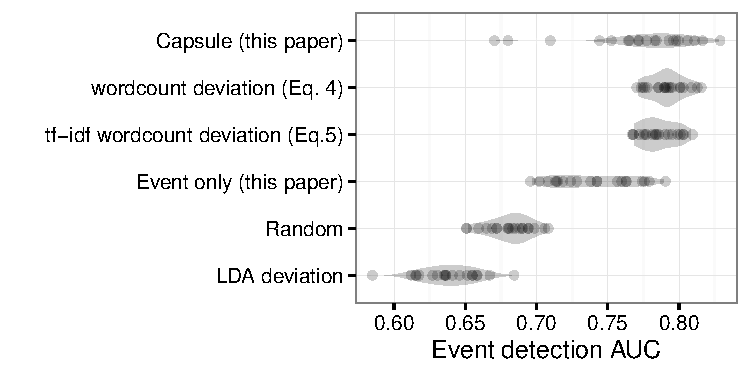
\includegraphics[width=\linewidth]{fig/sim_eventdetect.pdf}
\caption{Event detection performance using ten simulated data
  sets. Each dot represents the performance (\cref{eq:detection}) of
  a single method on a single data set; the shaded green area
  summarizes the distribution of performance for a single method.}
\label{fig:sim_eventdetect}
\end{figure}


\Cref{fig:sim_eventdetect} shows that Capsule outperforms all four
baseline methods. These results serve as a sanity check for the model
and its implementation.

%\footnote{The model was set with the same
%  number of topics $K=10$ and exponential decay $f$ used to simulate
%  the data.  More details on the decay function surround its formal
%  definition in \cref{eq:f}.}

\subsection{Identifying Relevant Messages}

For each data set, we created a list of the most relevant messages for
each time interval $t$ by computing $f(t_d, t)\,\epsilon_{dt}$ for
each message $d$ (using the simulated values of $\epsilon_{dt}$) and
ordering the messages accordingly. We then treated these ranked lists
of messages as ``ground truth'' and assessed how well Capsule and the
baseline methods were able to recover them.

For Capsule, we used our approximate inference algorithm to obtain a
fitted variational distribution for each simulated data set, and then,
for each time interval, ordered the messages according to $f(t_d,
t)\,\E[\epsilon_{dt}]$. For our second and third baselines, we ordered
the messages according per-document versions of \cref{eq:wordev} and
\cref{eq:tfidfwordev}---i.e.,
\begin{equation}
  m_{dt} = \sum_{v=1}^V \left\lvert n_{dv} - \frac{1}{D}\sum_{d=1}^D
  n_{dv} \right\rvert
\end{equation}
and
\begin{equation}
  m_{dt} = \sum_{v=1}^V \textrm{tf-idf}\,(v) \left\lvert n_{dv} - \frac{1}{D}\sum_{d=1}^D
  n_{dv} \right\rvert.
\end{equation}

For each data set, we compared each method's ranked list of documents
for each time interval to the corresponding ``ground-truth'' list, by
computing precision at 10 documents. The average precision for Capsule
was was 0.44, while the average precision for the ``event-only''
version of the model was 0.09. The other baselines recovered zero
relevant messages.

\section{Exploratory Analysis}
\label{sec:eval}

Capsule is intended to help analysts explore and understand their
data. In this section, we demonstrate its capabilities by analyzing a
corpus of over two million U.S. State Department cables from the
1970s.

\subsection{Data}

The National Archive collects diplomatic cables\footnote{The corpus also includes messages sent by diplomatic pouch, which we include in our analysis.} sent between the
U.S. State Department and its foreign embassies. We obtained a subset
of this corpus from the Central Foreign Policy Files at the National
Archives, via the History Lab at Columbia
University.\footnote{http://history-lab.org} The subset contains over
two million cables sent between 1973 and 1978. In addition to the text
of the cables, each message is labeled with its author (e.g., the
U.S. State Department, a particular embassy, or a named individual),
its recipients (often several), and the date the cable was sent. We
used a vocabulary of 6,293 terms and omitted cables with fewer than
three terms, resulting in 2,021,852 cables sent between 22,961
entities. We used weekly time intervals, as few cables were sent on
the weekends.

\subsection{Model Settings}

% what top-level shape/rate parameters did we use?

We ran our approximate inference algorithm for Capsule to obtain a
fitted variational distribution. We used $K=100$ general topics, the
exponential decay function in \cref{eq:f} with $\tau=4$, and top-level
hyperparameters $s=r=0.3$. With these settings, a single iteration of
the algorithm took about an hour.\footnote{Each iteration of our
  algorithm considers all messages. Modifying it to stochastically
  sample the data would reduce the time required to obtain an
  equivalent fitted variational distribution.}

\subsection{Quantitative Results}

Similar to the validation on simulated data discussed in \cref{sec:valid},
we can validate Capsule on this real-world data.  Here, we focus on event detection
and held-out data likelihood.

The History Lab at Columbia University provided us with a list of
thirty-nine well-known real-world events during that took place between 1973 and
1978. These events are present in at least one of six reputable
collections of historic events, such as the Office of the Historian's
Milestones in the History of U.S. Foreign
Relations.\footnote{\url{https://history.state.gov/milestones/1969-1976}}

We ran Capsule and baseline comparison methods to recover these events, and used the nDCG metric to evaluate the methods.  The nDCG metric is discounted cumulative gain,
\begin{equation}
\mbox{DCG} = \sum_{j=1}^T \frac{\mathbf{1}[\mbox{interval at rank $j$ in known events}]}{\log j},
\end{equation}
divided by the ideal DCG value, or
\begin{equation}
\mbox{nDCG} = \frac{\mbox{DCG}}{\mbox{ideal DCG}}.
\end{equation}
As shown in \Cref{table:cables:ndcg}, Capsule outperforms the baselines.
\begin{table*}[bt]
\centering
\begin{tabular}{l c}
\toprule
\textbf{Method} & \textbf{nDCG} \\
\midrule
Capsule & 0.693 \\
Average tf-idf weighted word count deviation & 0.652 \\
Average unweighted word count deviation & 0.642 \\
Single term maximum tf-idf weighted deviation & 0.561 \\
Random (10k ave) & 0.557 \\
Single term maximum unweighted deviation & 0.555 \\
%Total tf-idf weighted word count deviation; \Cref{eq:tfidfwordev}\footnotemark & 0.543626 \\
%Total unweighted word count deviation; \Cref{eq:wordev} & 0.540892 \\
\bottomrule
\end{tabular}
\caption{Evaluation of Capsule and comparison baselines on a collection of 39 real-world events.  Capsule performs best.}
\label{table:cables:ndcg}
\end{table*}
%\footnotetext{Note that this metric performed best on simulated data.}

Additionally, we computed held-out validation data likelihood on the model and each of its component parts; \Cref{table:cables:ll} shows that the full Capsule model captures the data better than any of its component parts individually.
\begin{table}[bt]
\centering
\begin{tabular}{l c c}
\toprule
\textbf{Model} & \textbf{LL, 10 iter.} & \textbf{LL, final} \\
\midrule
Full Capsule & -1.62e7 & -1.52e7 \\
Entity Topics Only & -1.64e7 & -- \\
General Topics Only & -1.71e7 & -1.53e7 \\
Event Only & -1.79e7 & -- \\
\bottomrule
\end{tabular}
\caption{Log likelihood (LL) computed on validation data at 10 iterations and at convergence---the event only and entity only models are small enough that they converge with very few iterations. The full Capsule model achieves the lowest log likelihood in both cases.}
\label{table:cables:ll}
\end{table}

\subsection{Exploration}

Having validated that Capsule can detect well-known real-world events, we now
turn to our primary goal---using Capsule to explore and understand a
corpus of messages, including discovering obscure, but potentially significant events.

\Cref{fig:cables_events} shows the ``eventness'' measure described in
\cref{sec:detecting} over time. High values---which are often
anomalous peaks---correspond to real-world events. One of the tallest
peaks occurs during the week of December 1, 1975, when the United
Nations General Assembly (UNGA) discussed omnibus decolonization. As
described in \cref{sec:detecting}, we can characterize this event by
computing $f(t_d, t)\,\E[\epsilon_{dt}]$ for each message $d$ and then
sorting the messages accordingly. \Cref{tab:decol} lists the
top-ranked cables.

\begin{table*}[tb]
\small
\centering
\begin{tabular}{cccl}
\toprule
$f(t_d, t) \E[\epsilon_{dt}]$ & \textbf{Date} & \textbf{Author Entity} & \textbf{Subject} \\
\midrule
4.60 & 1975-12-05 & Canberra & 30th UNGA: Item 23, Guam, Obmibus Decolonization and ... \\
4.26 & 1975-12-05 & Mexico & 30th UNGA-Item 23: Guam, Omnibus Decolonization and ... \\
4.21 & 1975-12-06 & State & 30th UNGA-Item 23: Guam, Omnibus Decolonization and ... \\
4.11 & 1975-12-03 & Dakar & 30th UNGA: Resolutions on American Samoa, Guam and ...\\
4.08 & 1975-12-04 & Monrovia & 30th UNGA: Item 23: Resolutions on decolonization and A...\\
\bottomrule
\end{tabular}
\caption{Top-ranked cables for the week of December 1, 1975, when the
  United Nations General Assembly discussed decolonization
  resolutions. Capsule accurately recovers cables related to this
  real-world event. Typos are intentionally copied from the data.}
\label{tab:decol}
\end{table*}

\begin{table*}[ht]
\small
\centering
\begin{tabular}{cccl}
\toprule
$f(t_d, t) \E[\epsilon_{dt}]$ & \textbf{Date} & \textbf{Author Entity} & \textbf{Subject} \\
\midrule
5.06 & 1975-05-15 & Sofia & Seizure of US merchant vessel by Cambodian forces \\
5.05 & 1975-05-15 & Dar es Salaam & Seizure of U.S.~merchant vessel by Cambodian forces \\
4.92 & 1975-05-16 & Lusaka & Seizure of US merchant vessel by Cambodian forces \\
4.61 & 1975-05-13 & Zagreb & Waiver request for INS Vienna visas Eagle name check... \\
4.59 & 1975-05-15 & State & eizure of US merchant Vessel by Cambodian forces \\
\bottomrule
\end{tabular}
\caption{Top-ranked cables for the week of May 12, 1975, when the
  S.S.~Mayaguez, an American merchant vessel, was captured. Capsule
  accurately recovers cables related to this real-world event. Typos
  are intentionally copied from the data.}
\label{tab:mayaguez}
\end{table*}

Another notable event was the seizure of the S.S.~Mayaguez, an
American merchant vessel, during May, 1975, at the end of the Vietnam
War. The top-ranked cables for this event are in
\cref{tab:mayaguez}. We can examine the individual cables to confirm
their relevancy and learn more about the event. For example, here is
the most relevant cable, according to Capsule:
\begin{shaded*} \tt{In absence of MFA Chief of Eighth Department Avramov, I
informed American desk officer Yankov of circumstances surrounding seizure
and recovery of merchant ship Mayaguez and its crew.  Yankov promised to
inform the Foreign Minister of US statement today  (May 15).
Batjer
}
\end{shaded*}


A third week of interest occurs in early July of 1976.  On July 4th, the US celebrated its Bicentennial, but on the same day, Israeli forces completed a hostage rescue mission---an Air France flight from Tel Aviv had been hijacked and taken to Entebbe, Uganda.  This event, like many events, is mostly discussed the week following the real-world event; relevant cables are shown in \Cref{sec:additional_results}, \Cref{tab:entebbe}.
The cable from Stockholm describing the ``Ugandan role in Air France hijacking'' begins with the following content, which reveals further information about the event.
\begin{shaded*} \tt{
1. We provided MFA Director of Political Affairs
Leifland with Evidence of Ugandan assistance to
hijackers contained in Ref A.  After reading material,{}
Leifland described it a ``quite good'', and said it{}
would be helpful for meeting MFA has scheduled for
early this morning to determine position GOS will take
at July 8 UNSC consideration of Israeli Rescue Operation. ...
}
\end{shaded*}
Capsule assumes that only one event occurs in each time interval---this example is a clear violation of this assumption, but it also demonstrates that the model successfully captures both events, even when they overlap.

In addition to characterizing known events, such as Operation Entebbe and the Mayaguez incident, Capsule identifies and characterizes obscure but potentially important events.  For example, it characterizes the kidnapping of Tenneco employees in 1974 and Operation Fluid Drive in 1976, both of which were previously unknown to our expert historian.  It also reveals that the UN held a Security Council meeting in Panama in 1973---our expert historian did not previously know that the UN had held any meetings in this country.

In addition to investigating events, Capsule can be used to explore the general themes of a corpus and entities' typical concerns.  Examples of general topics of conversation are shown in \Cref{sec:additional_results}, \Cref{tab:topics} and entity-exclusive topics are shown in \Cref{sec:additional_results}, \Cref{tab:entities}; these show us how entity topics absorb location-specific words, preventing these terms from overwhelming the general topics.

These exploratory results show that our model is successfully capturing when multiple entities are discussing the same subjects and that our model can be used to explore the underlying data by providing a structured scaffold from which to view the data.
